% Created by tikzDevice version 0.6.1 on 2016-07-16 10:57:14
% !TEX encoding = UTF-8 Unicode
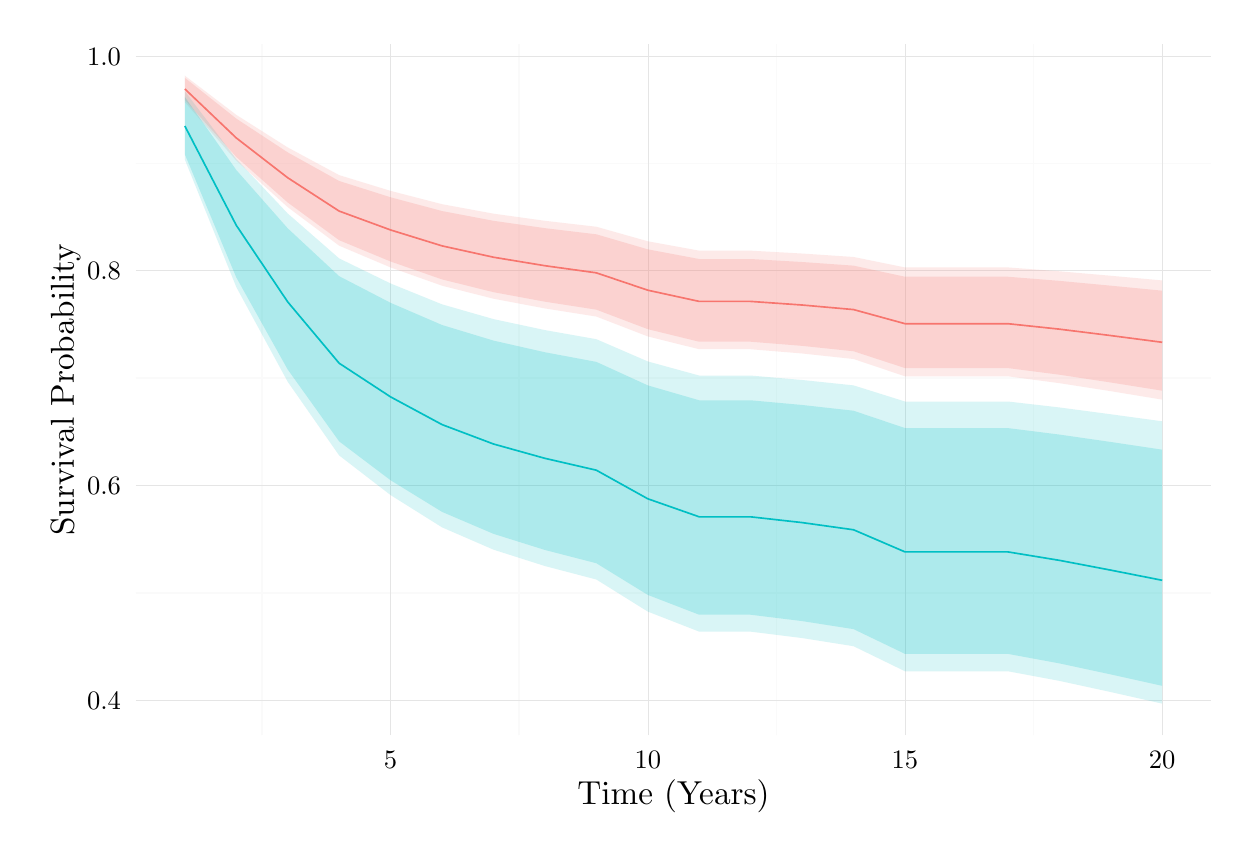
\begin{tikzpicture}[x=1pt,y=1pt]
\definecolor[named]{drawColor}{rgb}{0.00,0.00,0.00}
\definecolor[named]{fillColor}{rgb}{1.00,1.00,1.00}
\fill[color=fillColor,] (0,0) rectangle (433.62,289.08);
\begin{scope}
\path[clip] (  0.00,  0.00) rectangle (433.62,289.08);
\definecolor[named]{fillColor}{rgb}{0.00,0.00,0.00}
\end{scope}
\begin{scope}
\path[clip] (  0.00,  0.00) rectangle (433.62,289.08);
\definecolor[named]{fillColor}{rgb}{0.00,0.00,0.00}
\end{scope}
\begin{scope}
\path[clip] (  0.00,  0.00) rectangle (433.62,289.08);
\definecolor[named]{fillColor}{rgb}{0.00,0.00,0.00}
\end{scope}
\begin{scope}
\path[clip] (  0.00,  0.00) rectangle (433.62,289.08);
\definecolor[named]{fillColor}{rgb}{0.00,0.00,0.00}
\end{scope}
\begin{scope}
\path[clip] (  0.00,  0.00) rectangle (433.62,289.08);
\definecolor[named]{fillColor}{rgb}{0.00,0.00,0.00}
\end{scope}
\begin{scope}
\path[clip] (  0.00,  0.00) rectangle (433.62,289.08);
\definecolor[named]{fillColor}{rgb}{0.00,0.00,0.00}
\end{scope}
\begin{scope}
\path[clip] (  0.00,  0.00) rectangle (433.62,289.08);
\definecolor[named]{fillColor}{rgb}{0.00,0.00,0.00}
\end{scope}
\begin{scope}
\path[clip] (  0.00,  0.00) rectangle (433.62,289.08);
\definecolor[named]{fillColor}{rgb}{0.00,0.00,0.00}
\end{scope}
\begin{scope}
\path[clip] (  0.00,  0.00) rectangle (433.62,289.08);
\definecolor[named]{fillColor}{rgb}{0.00,0.00,0.00}
\end{scope}
\begin{scope}
\path[clip] (  0.00,  0.00) rectangle (433.62,289.08);
\definecolor[named]{fillColor}{rgb}{0.00,0.00,0.00}
\definecolor[named]{drawColor}{rgb}{1.00,1.00,1.00}
\definecolor[named]{fillColor}{rgb}{1.00,1.00,1.00}

\draw[color=drawColor,line width= 0.6pt,line cap=round,line join=round,fill=fillColor,] (  0.00,  0.00) rectangle (433.62,289.08);
\end{scope}
\begin{scope}
\path[clip] (  0.00,  0.00) rectangle (433.62,289.08);
\definecolor[named]{fillColor}{rgb}{0.00,0.00,0.00}
\end{scope}
\begin{scope}
\path[clip] (  0.00,  0.00) rectangle (433.62,289.08);
\definecolor[named]{fillColor}{rgb}{0.00,0.00,0.00}
\end{scope}
\begin{scope}
\path[clip] (  0.00,  0.00) rectangle (433.62,289.08);
\definecolor[named]{fillColor}{rgb}{0.00,0.00,0.00}
\end{scope}
\begin{scope}
\path[clip] ( 39.13, 33.48) rectangle (427.62,283.08);
\definecolor[named]{fillColor}{rgb}{0.00,0.00,0.00}
\definecolor[named]{fillColor}{rgb}{1.00,1.00,1.00}

\draw[fill=fillColor,draw opacity=0.00,] ( 39.13, 33.48) rectangle (427.62,283.08);
\definecolor[named]{drawColor}{rgb}{0.98,0.98,0.98}

\draw[color=drawColor,line width= 0.6pt,line join=round,fill opacity=0.00,] ( 39.13, 84.80) --
	(427.62, 84.80);

\draw[color=drawColor,line width= 0.6pt,line join=round,fill opacity=0.00,] ( 39.13,162.43) --
	(427.62,162.43);

\draw[color=drawColor,line width= 0.6pt,line join=round,fill opacity=0.00,] ( 39.13,240.05) --
	(427.62,240.05);

\draw[color=drawColor,line width= 0.6pt,line join=round,fill opacity=0.00,] ( 84.67, 33.48) --
	( 84.67,283.08);

\draw[color=drawColor,line width= 0.6pt,line join=round,fill opacity=0.00,] (177.61, 33.48) --
	(177.61,283.08);

\draw[color=drawColor,line width= 0.6pt,line join=round,fill opacity=0.00,] (270.55, 33.48) --
	(270.55,283.08);

\draw[color=drawColor,line width= 0.6pt,line join=round,fill opacity=0.00,] (363.49, 33.48) --
	(363.49,283.08);
\definecolor[named]{drawColor}{rgb}{0.90,0.90,0.90}

\draw[color=drawColor,line width= 0.2pt,line join=round,fill opacity=0.00,] ( 39.13, 45.99) --
	(427.62, 45.99);

\draw[color=drawColor,line width= 0.2pt,line join=round,fill opacity=0.00,] ( 39.13,123.61) --
	(427.62,123.61);

\draw[color=drawColor,line width= 0.2pt,line join=round,fill opacity=0.00,] ( 39.13,201.24) --
	(427.62,201.24);

\draw[color=drawColor,line width= 0.2pt,line join=round,fill opacity=0.00,] ( 39.13,278.86) --
	(427.62,278.86);

\draw[color=drawColor,line width= 0.2pt,line join=round,fill opacity=0.00,] (131.14, 33.48) --
	(131.14,283.08);

\draw[color=drawColor,line width= 0.2pt,line join=round,fill opacity=0.00,] (224.08, 33.48) --
	(224.08,283.08);

\draw[color=drawColor,line width= 0.2pt,line join=round,fill opacity=0.00,] (317.02, 33.48) --
	(317.02,283.08);

\draw[color=drawColor,line width= 0.2pt,line join=round,fill opacity=0.00,] (409.96, 33.48) --
	(409.96,283.08);
\definecolor[named]{drawColor}{rgb}{0.97,0.46,0.43}
\definecolor[named]{fillColor}{rgb}{0.97,0.46,0.43}

\draw[color=drawColor,line width= 0.6pt,line join=round,] ( 56.79,266.93) --
	( 75.38,249.23) --
	( 93.96,234.85) --
	(112.55,222.80) --
	(131.14,215.98) --
	(149.73,210.23) --
	(168.32,206.13) --
	(186.90,203.06) --
	(205.49,200.49) --
	(224.08,194.21) --
	(242.67,190.16) --
	(261.26,190.16) --
	(279.84,188.86) --
	(298.43,187.21) --
	(317.02,182.11) --
	(335.61,182.11) --
	(354.20,182.11) --
	(372.79,180.14) --
	(391.37,177.82) --
	(409.96,175.39);
\definecolor[named]{drawColor}{rgb}{0.00,0.75,0.77}
\definecolor[named]{fillColor}{rgb}{0.00,0.75,0.77}

\draw[color=drawColor,line width= 0.6pt,line join=round,] ( 56.79,253.55) --
	( 75.38,217.66) --
	( 93.96,189.99) --
	(112.55,167.83) --
	(131.14,155.66) --
	(149.73,145.65) --
	(168.32,138.64) --
	(186.90,133.46) --
	(205.49,129.17) --
	(224.08,118.84) --
	(242.67,112.32) --
	(261.26,112.32) --
	(279.84,110.24) --
	(298.43,107.64) --
	(317.02, 99.65) --
	(335.61, 99.65) --
	(354.20, 99.65) --
	(372.79, 96.60) --
	(391.37, 93.06) --
	(409.96, 89.39);
\definecolor[named]{fillColor}{rgb}{0.97,0.46,0.43}

\draw[fill=fillColor,fill opacity=0.15,draw opacity=0.00,] ( 56.79,271.73) --
	( 75.38,257.57) --
	( 93.96,245.80) --
	(112.55,235.80) --
	(131.14,230.10) --
	(149.73,225.29) --
	(168.32,221.87) --
	(186.90,219.29) --
	(205.49,217.14) --
	(224.08,211.89) --
	(242.67,208.50) --
	(261.26,208.50) --
	(279.84,207.46) --
	(298.43,206.22) --
	(317.02,202.44) --
	(335.61,202.44) --
	(354.20,202.44) --
	(372.79,201.05) --
	(391.37,199.43) --
	(409.96,197.74) --
	(409.96,154.67) --
	(391.37,157.73) --
	(372.79,160.63) --
	(354.20,163.10) --
	(335.61,163.10) --
	(317.02,163.10) --
	(298.43,169.35) --
	(279.84,171.35) --
	(261.26,172.88) --
	(242.67,172.88) --
	(224.08,177.51) --
	(205.49,184.69) --
	(186.90,187.63) --
	(168.32,191.14) --
	(149.73,195.84) --
	(131.14,202.44) --
	(112.55,210.30) --
	( 93.96,224.23) --
	( 75.38,241.07) --
	( 56.79,262.19) --
	cycle;
\definecolor[named]{fillColor}{rgb}{0.00,0.75,0.77}

\draw[fill=fillColor,fill opacity=0.15,draw opacity=0.00,] ( 56.79,266.11) --
	( 75.38,241.61) --
	( 93.96,221.94) --
	(112.55,205.70) --
	(131.14,196.64) --
	(149.73,189.10) --
	(168.32,183.77) --
	(186.90,179.80) --
	(205.49,176.51) --
	(224.08,168.47) --
	(242.67,163.37) --
	(261.26,163.37) --
	(279.84,161.77) --
	(298.43,159.82) --
	(317.02,153.99) --
	(335.61,153.99) --
	(354.20,153.99) --
	(372.79,151.85) --
	(391.37,149.38) --
	(409.96,146.84) --
	(409.96, 44.82) --
	(391.37, 49.01) --
	(372.79, 53.05) --
	(354.20, 56.52) --
	(335.61, 56.52) --
	(317.02, 56.52) --
	(298.43, 65.57) --
	(279.84, 68.52) --
	(261.26, 70.83) --
	(242.67, 70.83) --
	(224.08, 78.08) --
	(205.49, 89.67) --
	(186.90, 94.54) --
	(168.32,100.46) --
	(149.73,108.52) --
	(131.14,120.18) --
	(112.55,134.51) --
	( 93.96,161.13) --
	( 75.38,195.36) --
	( 56.79,241.41) --
	cycle;
\definecolor[named]{fillColor}{rgb}{0.97,0.46,0.43}

\draw[fill=fillColor,fill opacity=0.20,draw opacity=0.00,] ( 56.79,270.96) --
	( 75.38,256.22) --
	( 93.96,244.02) --
	(112.55,233.68) --
	(131.14,227.79) --
	(149.73,222.82) --
	(168.32,219.29) --
	(186.90,216.63) --
	(205.49,214.41) --
	(224.08,208.98) --
	(242.67,205.48) --
	(261.26,205.48) --
	(279.84,204.40) --
	(298.43,203.09) --
	(317.02,199.08) --
	(335.61,199.08) --
	(354.20,199.08) --
	(372.79,197.59) --
	(391.37,195.85) --
	(409.96,194.04) --
	(409.96,157.90) --
	(391.37,160.86) --
	(372.79,163.68) --
	(354.20,166.07) --
	(335.61,166.07) --
	(317.02,166.07) --
	(298.43,172.15) --
	(279.84,174.10) --
	(261.26,175.59) --
	(242.67,175.59) --
	(224.08,180.13) --
	(205.49,187.18) --
	(186.90,190.06) --
	(168.32,193.50) --
	(149.73,198.11) --
	(131.14,204.58) --
	(112.55,212.28) --
	( 93.96,225.91) --
	( 75.38,242.37) --
	( 56.79,262.95) --
	cycle;
\definecolor[named]{fillColor}{rgb}{0.00,0.75,0.77}

\draw[fill=fillColor,fill opacity=0.20,draw opacity=0.00,] ( 56.79,264.06) --
	( 75.38,237.64) --
	( 93.96,216.58) --
	(112.55,199.28) --
	(131.14,189.65) --
	(149.73,181.64) --
	(168.32,176.00) --
	(186.90,171.79) --
	(205.49,168.31) --
	(224.08,159.82) --
	(242.67,154.43) --
	(261.26,154.43) --
	(279.84,152.74) --
	(298.43,150.66) --
	(317.02,144.39) --
	(335.61,144.39) --
	(354.20,144.39) --
	(372.79,142.05) --
	(391.37,139.37) --
	(409.96,136.59) --
	(409.96, 51.25) --
	(391.37, 55.38) --
	(372.79, 59.37) --
	(354.20, 62.80) --
	(335.61, 62.80) --
	(317.02, 62.80) --
	(298.43, 71.74) --
	(279.84, 74.65) --
	(261.26, 76.94) --
	(242.67, 76.94) --
	(224.08, 84.11) --
	(205.49, 95.55) --
	(186.90,100.35) --
	(168.32,106.18) --
	(149.73,114.11) --
	(131.14,125.54) --
	(112.55,139.58) --
	( 93.96,165.57) --
	( 75.38,198.84) --
	( 56.79,243.33) --
	cycle;
\end{scope}
\begin{scope}
\path[clip] (  0.00,  0.00) rectangle (433.62,289.08);
\definecolor[named]{fillColor}{rgb}{0.00,0.00,0.00}
\end{scope}
\begin{scope}
\path[clip] (  0.00,  0.00) rectangle (433.62,289.08);
\definecolor[named]{fillColor}{rgb}{0.00,0.00,0.00}
\end{scope}
\begin{scope}
\path[clip] (  0.00,  0.00) rectangle (433.62,289.08);
\definecolor[named]{fillColor}{rgb}{0.00,0.00,0.00}
\end{scope}
\begin{scope}
\path[clip] (  0.00,  0.00) rectangle (433.62,289.08);
\definecolor[named]{fillColor}{rgb}{0.00,0.00,0.00}
\end{scope}
\begin{scope}
\path[clip] (  0.00,  0.00) rectangle (433.62,289.08);
\definecolor[named]{fillColor}{rgb}{0.00,0.00,0.00}
\end{scope}
\begin{scope}
\path[clip] (  0.00,  0.00) rectangle (433.62,289.08);
\definecolor[named]{fillColor}{rgb}{0.00,0.00,0.00}
\definecolor[named]{drawColor}{rgb}{0.00,0.00,0.00}

\node[color=drawColor,anchor=base east,inner sep=0pt, outer sep=0pt, scale=  0.96] at ( 33.73, 42.68) {0.4%
};

\node[color=drawColor,anchor=base east,inner sep=0pt, outer sep=0pt, scale=  0.96] at ( 33.73,120.31) {0.6%
};

\node[color=drawColor,anchor=base east,inner sep=0pt, outer sep=0pt, scale=  0.96] at ( 33.73,197.93) {0.8%
};

\node[color=drawColor,anchor=base east,inner sep=0pt, outer sep=0pt, scale=  0.96] at ( 33.73,275.56) {1.0%
};
\end{scope}
\begin{scope}
\path[clip] (  0.00,  0.00) rectangle (433.62,289.08);
\definecolor[named]{fillColor}{rgb}{0.00,0.00,0.00}
\end{scope}
\begin{scope}
\path[clip] (  0.00,  0.00) rectangle (433.62,289.08);
\definecolor[named]{fillColor}{rgb}{0.00,0.00,0.00}
\end{scope}
\begin{scope}
\path[clip] (  0.00,  0.00) rectangle (433.62,289.08);
\definecolor[named]{fillColor}{rgb}{0.00,0.00,0.00}
\end{scope}
\begin{scope}
\path[clip] (  0.00,  0.00) rectangle (433.62,289.08);
\definecolor[named]{fillColor}{rgb}{0.00,0.00,0.00}
\end{scope}
\begin{scope}
\path[clip] (  0.00,  0.00) rectangle (433.62,289.08);
\definecolor[named]{fillColor}{rgb}{0.00,0.00,0.00}
\end{scope}
\begin{scope}
\path[clip] (  0.00,  0.00) rectangle (433.62,289.08);
\definecolor[named]{fillColor}{rgb}{0.00,0.00,0.00}
\end{scope}
\begin{scope}
\path[clip] (  0.00,  0.00) rectangle (433.62,289.08);
\definecolor[named]{fillColor}{rgb}{0.00,0.00,0.00}
\end{scope}
\begin{scope}
\path[clip] (  0.00,  0.00) rectangle (433.62,289.08);
\definecolor[named]{fillColor}{rgb}{0.00,0.00,0.00}
\end{scope}
\begin{scope}
\path[clip] (  0.00,  0.00) rectangle (433.62,289.08);
\definecolor[named]{fillColor}{rgb}{0.00,0.00,0.00}
\end{scope}
\begin{scope}
\path[clip] (  0.00,  0.00) rectangle (433.62,289.08);
\definecolor[named]{fillColor}{rgb}{0.00,0.00,0.00}
\end{scope}
\begin{scope}
\path[clip] (  0.00,  0.00) rectangle (433.62,289.08);
\definecolor[named]{fillColor}{rgb}{0.00,0.00,0.00}
\end{scope}
\begin{scope}
\path[clip] (  0.00,  0.00) rectangle (433.62,289.08);
\definecolor[named]{fillColor}{rgb}{0.00,0.00,0.00}
\definecolor[named]{drawColor}{rgb}{0.00,0.00,0.00}

\node[color=drawColor,anchor=base,inner sep=0pt, outer sep=0pt, scale=  0.96] at (131.14, 21.46) {5%
};

\node[color=drawColor,anchor=base,inner sep=0pt, outer sep=0pt, scale=  0.96] at (224.08, 21.46) {10%
};

\node[color=drawColor,anchor=base,inner sep=0pt, outer sep=0pt, scale=  0.96] at (317.02, 21.46) {15%
};

\node[color=drawColor,anchor=base,inner sep=0pt, outer sep=0pt, scale=  0.96] at (409.96, 21.46) {20%
};
\end{scope}
\begin{scope}
\path[clip] (  0.00,  0.00) rectangle (433.62,289.08);
\definecolor[named]{fillColor}{rgb}{0.00,0.00,0.00}
\end{scope}
\begin{scope}
\path[clip] (  0.00,  0.00) rectangle (433.62,289.08);
\definecolor[named]{fillColor}{rgb}{0.00,0.00,0.00}
\end{scope}
\begin{scope}
\path[clip] (  0.00,  0.00) rectangle (433.62,289.08);
\definecolor[named]{fillColor}{rgb}{0.00,0.00,0.00}
\end{scope}
\begin{scope}
\path[clip] (  0.00,  0.00) rectangle (433.62,289.08);
\definecolor[named]{fillColor}{rgb}{0.00,0.00,0.00}
\definecolor[named]{drawColor}{rgb}{0.00,0.00,0.00}

\node[color=drawColor,anchor=base,inner sep=0pt, outer sep=0pt, scale=  1.20] at (233.37,  8.40) {Time (Years)%
};
\end{scope}
\begin{scope}
\path[clip] (  0.00,  0.00) rectangle (433.62,289.08);
\definecolor[named]{fillColor}{rgb}{0.00,0.00,0.00}
\end{scope}
\begin{scope}
\path[clip] (  0.00,  0.00) rectangle (433.62,289.08);
\definecolor[named]{fillColor}{rgb}{0.00,0.00,0.00}
\definecolor[named]{drawColor}{rgb}{0.00,0.00,0.00}

\node[rotate= 90.00,color=drawColor,anchor=base,inner sep=0pt, outer sep=0pt, scale=  1.20] at ( 16.66,158.28) {Survival Probability%
};
\end{scope}
\begin{scope}
\path[clip] (  0.00,  0.00) rectangle (433.62,289.08);
\definecolor[named]{fillColor}{rgb}{0.00,0.00,0.00}
\end{scope}
\begin{scope}
\path[clip] (  0.00,  0.00) rectangle (433.62,289.08);
\definecolor[named]{fillColor}{rgb}{0.00,0.00,0.00}
\end{scope}
\begin{scope}
\path[clip] (  0.00,  0.00) rectangle (433.62,289.08);
\definecolor[named]{fillColor}{rgb}{0.00,0.00,0.00}
\end{scope}
\begin{scope}
\path[clip] (  0.00,  0.00) rectangle (433.62,289.08);
\definecolor[named]{fillColor}{rgb}{0.00,0.00,0.00}
\end{scope}
\end{tikzpicture}
